\documentclass[hidelinks]{report}
\usepackage{amsmath, amssymb, amsthm}
\usepackage{thmtools}
\usepackage{algorithm}
\usepackage{algpseudocode}
\usepackage{nameref, hyperref, cleveref}
\usepackage{tikz}
\usepackage[shortlabels]{enumitem}
\usepackage{todonotes}
\usepackage{enumitem}
\usepackage{subcaption}

\usepackage[
backend=biber,
style=alphabetic,
sorting=ynt
]{biblatex}
\addbibresource{refs.bib}

\setenumerate{itemsep=-.5ex}

\usetikzlibrary{positioning, arrows.meta, shapes}

\newcommand{\Ac}{\mathcal{A}}  % alphabet
\newcommand{\Lc}{\mathcal{L}}  % label function
\newcommand{\Gc}{\mathcal{G}}  % labeled graph
\newcommand{\Hc}{\mathcal{H}}  % labeled graph
\newcommand{\Vc}{\mathcal{V}}
\newcommand{\Ec}{\mathcal{E}}
\newcommand{\Bc}{\mathcal{B}}
\newcommand{\Fc}{\mathcal{F}}
\newcommand{\GtH}{{\Gc^\to\Hc}}
\newcommand{\shift}[1]{\mathsf{X}_{#1}}
\newcommand{\term}[1]{\textit{#1}}

\usepackage[bitstream-charter, cal=cmcal]{mathdesign}

\theoremstyle{definition}
\declaretheorem[numberwithin=chapter]{theorem}
\declaretheorem[sibling=theorem]{lemma}
\declaretheorem[sibling=theorem]{example}
\declaretheorem[sibling=theorem]{proposition}
\declaretheorem[sibling=theorem]{definition}
\declaretheorem[sibling=theorem]{corollary}

\renewcommand{\baselinestretch}{1.2}
\setlength{\parskip}{.05em}

\title{Towards algorithms for reducible presentations of sofic shifts}
\author{Justin Cai}

\begin{document}

\begin{titlepage}
    \raggedright
    \vspace*{3cm}
    {\fontsize{30}{100}\selectfont 
    \textbf{Towards algorithms for reducible presentations of sofic shifts}}

    \vspace{.75cm}
    \LARGE by Justin Cai

    \vspace{.75cm}
    \Large April 2020

    \vspace{4cm}
    \normalsize \textit{A thesis submitted in partial fullfillment of
    the requirements for the degree of Bachelor of Science in the Deparment of Computer Science \\
    at the University of Colorado Boulder  }
\end{titlepage}

\begin{abstract}
    \thispagestyle{plain}
    \pagenumbering{roman}
    Given an irreducible presentation of a sofic shift, it is well known 
    that there is a procedure that yields a presentation with the fewest
    vertices among all presentations of the shift in polynomial time. However, 
    given a reducible presentation,
    the previous procedure does not necessarily yield such a minimal presentation.
    If the reducible presentation presents an irreducible shift, 
    then an irreducible presentation that presents the whole shift itself
    can be found within this presentation,
    so one could minimize these by these presentations by finding this 
    component within the presentation. However, without knowing in advance
    if presentation presented an irreducible shift or not, this procedure
    would not work, so an algorithm for testing that is desirable. 
    In this thesis, we present progress towards such an algorithm.
\end{abstract}

\renewcommand{\abstractname}{Acknowledgements}
\begin{abstract}
    \setcounter{page}{2}
    \thispagestyle{plain}
Raf, if I didn't take your theory of computation course, I probably would've 
never gotten to the the level of appreciation and joy for mathematics and 
theoretical computer science I have now (or at least taken a lot longer),
so thank you for your class, introducing me to 
symbolic dynamics, being willing to advise me, and being a great advisor overall.

\vspace{.5cm}\noindent Jem and Josh, thank you for volunteering your time to be on my committee.
It is much appreciated!

\vspace{.5cm}\noindent STARBURTS\footnote{
\textbf{S}uper 
\textbf{T}errific 
\textbf{A}wesome 
\textbf{R}adical 
\textbf{B}rilliant 
\textbf{U}rban 
\textbf{R}eally 
\textbf{S}emantic 
\textbf{T}echnical 
\textbf{S}uperstars}, thanks for being 
a great bunch of friends this semester (and for listening to me talk about theory 
of computation for three hours).
\end{abstract}

\setcounter{page}{3}
\tableofcontents

\chapter{Introduction}

\pagenumbering{arabic}


In an effort to to sharpen the dividing 
line between classical differential analysis and abstract symbolic analysis
used frequently in the study of recurrence and transitivity in dynamical systems, 
and Morse and Hedlund named the field of symbolic dynamics in their eponymous 
1938 paper \cite{morse1938symbolic}. Shift spaces (or simply shifts), the main object 
of study in symbolic dynamics, are sets unending sequences over a finite set of 
symbols in which certain forbidden finite sequences (know as forbidden words)
are not allowed to appear in the unending sequences. If a shift space has a finite set of 
forbidden words that describe it, then the shift space is known as a shift 
of finite type (SFT). In addition to being characterized by a 
finite list of forbidden words, SFTs also have a representation in a graphical 
form, in the sense that all the unending sequences of SFTs can be 
described by reading off the vertices in an infinite walk around a graph.
Sofic shifts were introduced by \cite{weiss1973subshifts} as the smallest 
class of shift spaces containing every SFT and which were closed under 
factor codes. However, it was clear that sofic 
shifts were exactly the shifts described by infinite walks around 
a labeled graph.\footnote{The word sofic is derived from the Hebrew word 
for finite \cite{lind1995introduction}, which an apt name as sofic shifts 
generalize shifts of \textit{finite} type while still having a finite 
representation though a labeled graph. Additionally, a shift space is sofic 
iff it has a finite number of follower sets, which is closely related 
to the Myhill-Nerode theorem from automata theory.}

The labeled graphs that described sofic shifts, referred to hereafter as presentations
of a sofic shift, are not unique, in the sense that many different presentations 
can present the same sofic shift. Fischer \cite{fischer1975sofic} was interested in 
irreducible sofic shifts (what he called transitive), and shows that such sofic shifts admit 
a unique minimal deterministic presentation (with respect to number of vertices in the presentation).
\cite{jonoska1994minimal} further characterized these minimal presentations.
Sofic shifts that are reducible (i.e. not irreducible) do not 
necessarily admit a unique minimal presentation, which can be seen in \cite{jonoska1996sofic},  
where two presentations of a SFT were given that had the smallest number of 
vertices among all presentation of the SFT, but the presentations were distinct.
In the same paper, Jonoska characterized sofic shifts that had
synchronizing deterministic presentations in terms of the syntactic monoid 
of the language of the shift, and showed that any sofic shift having 
a synchronizing deterministic presentation necessarily had a unique 
minimal one.

The algorithms that exist for minimizing presentations of sofic shift 
seem to only be a well-known procedure that is essentially 
based on DFA minimization \cite{hopcroft2001introduction,lind1995introduction}. 
However, this algorithm is only guaranteed to yield the minimal presentation when 
given an irreducible presentation (where irreducibility of a presentation is a property
of the presentation being ``connected'').
Irreducible presentations present irreducible shifts, but reducible presentations do not 
necessarily present reducible shifts (i.e. a reducible presentation can present 
an irreducible shift). It 
has been essentially noted in \cite{jonoska1996sofic,marcus1991bounds,jonoska1994minimal} 
that presentations that present irreducible sofic shifts contain an irreducible subgraph 
which present the whole shift itself. Therefore, if you you 
knew that a presentation presented an irreducible shift, a procedure
to yield the minimal presentation would be to select the irreducible subgraph 
that presents the shift, and then further minimizing that (if necessary). However, 
an algorithm for deciding whether any presentation presents an irreducible shift 
seems to be mentioned nowhere in the literature. In this thesis, we work towards such an algorithm.


\chapter{Preliminaries}

In this section we introduce basic concepts from symbolic dynamics. 
Definitions and notation follow \cite{lind1995introduction} closely.

\begin{definition}
    Let \(\Ac\) be a finite set. The \term{full \(\Ac\)-shift} is the set \(\Ac^\mathbb{Z}\) of all 
    bi-infinite sequences over \(\Ac\) (i.e. functions from \(\mathbb{Z}\) to \(\Ac\), hence the 
    usual notation for the set of all functions from \(\mathbb{Z}\) to \(\Ac\)).
    Elements in \(\Ac^\mathbb{Z}\) are called \term{points}.
\end{definition}

A \term{word} is a finite sequence of letters over some alphabet \(\Ac\). We use 
\(\epsilon\) to denote the empty word.
Let \(x=(x_i)_{i \in \mathbb{Z}}\) be a bi-infinite sequence. For \(i \leq j\), the word from the 
\(i\)th coordinate to the \(j\)th coordinate is denoted \[x_{[i,j]} \triangleq x_i x_{i+1} \dots x_{j}.\]

\begin{definition}
    Let \(\Fc\) be a set of words over some alphabet, called the \term{forbidden words}.
    A \term{shift space} (or simply \term{shift}) is a subset \(\shift{\Fc}\)
    of some full shift \(\Ac^\mathbb{Z}\) such that none of the forbidden words appear in any point of the shift space.
    That is,
    \[\shift{\Fc} \triangleq \big\{ \; (x_i)_{i \in \mathbb{Z}} \in \Ac^\mathbb{Z} \; : \; \forall i, j \in \mathbb{Z}, i < j \quad  x_{[i,j]} \notin \Fc \; \big\}.\]
\end{definition}

If \(X\) and \(Y\) are shift spaces and \(X \subseteq Y\), then we say \(X\) is a \term{subshift} of \(Y\).
We can see that \(\Ac^\mathbb{Z}\) is a shift space by taking \(\Fc = \varnothing\), so as 
every shift space is a subset of a full shift, so shift spaces are sometimes synonymously referred to 
as subshifts.

\begin{definition}
    Let \(X\) be a shift space. The \term{language of \(X\)} is the set 
    \[\Bc(X) = \{ x_{[i,j]} : x \in X, i, j \in \mathbb{Z}, i < j\}\]
    of nonempty words that appear in some point in \(X\).
\end{definition}

Instead of specifying what words are forbidden in a shift space, we can characterize 
shift spaces by their languages. If \(L \subseteq \Ac^+\)\footnote{
    \(\Ac^*\) denotes the set of all words over \(\Ac\) including \(\epsilon\);
    \(\Ac^+\) is \(\Ac^*\) without \(\epsilon\).
} is a set of nonempty words, then 
we say \(L\) is \term{factorial} if for every word \(w \in L\), then every nonempty subword 
is in \(L\). We say \(L\) is \term{prolongable} if there for every word \(w \in L\), 
there are nonempty words \(u, v \in L\) such that \(uwv \in L\).

\begin{theorem}[name=\cite{lind1995introduction}]
    If \(L \subseteq \Ac^+\) is a set of nonempty words, then \(L = \Bc(X)\) for some 
    shift space \(X\) if and only if \(L\) is factorial and prolongable. 
    Furthermore, for any shift space, \(X = \shift{\Ac^+\backslash\Bc(X)}\), so 
    two shift spaces are equal if and only if their languages are equal.
\end{theorem}

The following theorem will be useful for our discussion and is simple enough to 
most likely well known, but no reference was found for it, so we provide a proof.

\begin{theorem}
    If \(X\) and \(Y\) are shift spaces, then \(X \subseteq Y\) if and only if \(\Bc(X) \subseteq \Bc(Y)\).
\end{theorem}

\begin{proof}
    Suppose \(X \subseteq Y\). If \(w \in \Bc(X)\), then \(w\) occurs in some point 
    \(x \in X\). But \(x \in Y\) as \(X \subseteq Y\), so \(w\) occurs in some point 
    in \(Y\). Therefore, \(w \in \Bc(Y)\).

    Conversely, suppose \(\Bc(X) \subseteq \Bc(Y)\). If \(x \in X\), then every 
    word occuring in \(x\) is in \(\Bc(X)\). But \(\Bc(X) \subseteq \Bc(Y)\), 
    so every word occuring in \(x\) is in \(\Bc(Y)\), so \(x \in Y\).
\end{proof}

\begin{definition}
    Let \(X\) be a shift space. If \(u, v \in \Bc(X)\) and there 
    is a word \(w \in \Bc(X)\) such that \(uwv \in \Bc(X)\), then we say 
    \(w\) joins \(u\) and \(v\). If for every pair of words in \(u, v \in \Bc(X)\) 
    there is a word \(w\) joining \(u\) and \(v\), then we say X is \term{irreducible}.
    Otherwise, we say \(X\) is \term{reducible}.
\end{definition}

\begin{example}
    A typical shift space we will see is the \term{even shift}. We define 
    the even shift to be the set of bi-infinite sequences over \(\{0, 1\}\)
    such that between any two \(1\)'s, there is an even number of \(0\)'s. That 
    is, the forbidden blocks are \(\{10^{2k+1}1 : k \geq 0\}\). The even shift is 
    also irreducible, which can be easily seen to see after we introduce 
    presentations of sofic shifts. 

    Another shift space is the \term{\(010\)-shift}, which are 
    the bi-infinite sequences over \(\{0, 1\}\) such that \(1\) only appears at most once. 
    We can describe the shift using the forbidden blocks \(\{10^k1 : k \geq 0\}\). This 
    shift space is reducible, as \(1\) is in the language, but if there 
    were a word joining \(1\) and \(1\), the the the resulting 
    word would contain a forbidden word, so there can be no word joining \(1\) and \(1\).
\end{example}

\begin{definition}
    A \term{graph}\footnote{
        In our discussion, a graph really means a directed multigraph; there 
        can be multiple edges between the same two vertices.
    } \(G\) is a \(4\)-tuple \(G = (\Vc, \Ec, i, t)\), where \(\Vc\) is a finite 
    set of \term{vertices}, \(\Ec\) is a finite set of \term{edges}, and \(i : \Ec \to \Vc\) and 
    \(t : \Ec \to \Vc\) are functions assigning an \term{initial} and \term{terminating} vertex for 
    each edge, respectivley. For an arbitrary graph \(G\), let 
    \(\Vc_G\), \(\Ec_G\), \(i_G\), and \(t_G\) denote the graph's vertices, edges, and 
    intial and terminating vertex functions, respectivley. 
\end{definition}


\begin{definition}
    Let \(G\) be a graph. A \term{bi-infinite walk in \(G\)} is 
    a bi-infinite sequence \(x\) over the edges of \(G\) such that \(t(x_i) = i(x_{i+1})\)
    for all \(i \in \mathbb{Z}\).
    The set \(\shift{G}\) of all bi-infinite 
    walks on \(G\) (called the \term{edge shift}) is denoted
    \[\shift{G} \triangleq \big\{ \; (x_i)_{i \in \mathbb{Z}} \in \Ec^\mathbb{Z} \; : \; \forall i \in \mathbb{Z} \quad t(x_i) = i(x_{i+1}) \; \big\}. \]
\end{definition}

\begin{theorem}[name=\cite{lind1995introduction}]
    If \(G\) is a graph, then \(\shift{G}\) is a shift space.
\end{theorem}

Let \(G\) be a graph. A \term{path in \(G\)} is a nonempty finite sequence of edges \(\pi = e_1 \dots e_n\) such that \(t(e_i) = i(e_{i+1})\) for all \(i < n\).
If \(I\) is a vertex in \(G\), we say a path \term{starts at \(I\)} if \(i(e_1) = I\). Similarly, 
we say a path \term{ends at \(I\)} if \(t(e_n) = I\).

Notice that every word in \(\Bc(\shift{G})\) is in \(G\), but every path in G is 
not necessarily a word in \(\Bc(\shift{G})\). Call a vertex \term{stranded} if 
there is no edge starting at \(I\) or  ending at \(I\). No bi-infinite walk can go 
through a stranded vertex, because a bi-infinite path must always have a ``next''
or ``previous'' vertex, and stranded vertices are exactly the vertices which have none.
If \(G\) has no stranded vertices, then we call \(G\) \term{essential}. Every 
non-essential graph can be made essential by removing the stranded vertices, and 
the resulting graph will have still have the same edge shift. Then, if \(G\) 
is essential, then every path in \(G\) is necessarily a word in \(\Bc(\shift{G})\). 
Thus, it simplifies our disucssion to work with essential graphs, as 
it allows us to paths and words in the language of an edge shift synonymously. 

If \(G\) is a graph and \(I\) and \(J\)
are vertices in \(G\), then we say \term{\(J\) is reachable from \(I\)}
if there is a path starting at \(I\) and ending at \(J\). We say \(G\) is \term{irreducible}
every pair of vertices reachable from each other. Otherwise, we say \(G\) is \term{reducible}. 
Every irreducible graph is necessarily essential. If \(G\) is irreducible, then 
it it not too hard to see that \(\shift{G}\) is irreducible. However, 
as we will discuss in the next section \(\shift{G}\) is not necessarily reducible 
if \(G\) is reducible.

\begin{definition}
    A \term{labeled graph} \(\Gc\) is a pair \((G, \Lc)\), where \(G\) is a graph and \(\Lc : \Ec \to \Ac\) is the 
    \term{labeling function} from the edges of \(G\) onto some finite alphabet \(\Ac\). We 
    refer to \(G\) as the \term{underlying graph}.
    As we did with graphs, if \(\Gc\) is an arbitrary labeled graph, then 
    let \(\Vc_\Gc, \Ec_\Gc, i_\Gc,\) and \(t_\Gc\) denote the vertices, edges, 
    initial and terminating vertex functions of the underlying graph. Additionally,
    let \(\Lc_\Gc\) denote the labeling function and \(\Ac_\Gc\) denote the set 
    of labels appearing in \(\Gc\) (i.e. the image of \(\Lc_\Gc\)).
\end{definition}

If \(\Gc\) is a labeled graph, then we will let \(\Gc\) inherit properties of its underlying 
graph. Specifically, we say \(\Gc\) is essential if its underlying graph is essential, 
\(\Gc\) is irreducible if its underlying graph is irreducible, and \(\Gc\) is reducible 
if its underlying graph is reducible, and so on. 

\begin{definition}
    Let \(\Gc = (G, \Lc)\) be a labeled graph. If \(x\) is a bi-infinite walk in \(G\), 
    then the \term{label of \(x\)} is the bi-infinite sequence \((\xi_i)_{i \in \mathbb{Z}}\), 
    where \(\xi_i = \Lc(x_i)\) for all \(i \in \mathbb{Z}\). The set of all the labels of 
    bi-infinite walks in \(G\) is denoted
    \[\shift{\Gc} \triangleq \big\{ \; (\xi_i)_{i \in \mathbb{Z}} : \xi_i = \Lc(x_i), x \in \shift{G} \; \big\}.  \]
\end{definition}

\begin{theorem}[name=\cite{lind1995introduction}]
    If \(\Gc\) is a labeled graph, then \(\shift{\Gc}\) is a shift space.
\end{theorem}

If \(X\) is a shift space and \(X = \shift{\Gc}\) for some labeled graph \(\Gc\), 
then we say \(X\) is a \term{sofic shift}. We say \term{\(\Gc\) presents \(X\)}, 
and will also refer to \(\Gc\) as a \term{presentation of \(X\)}. 

Let \(\Gc\) be a labeled graph. 
If \(\pi = e_1 \dots e_n\) is a path in \(\Gc\), then we will abuse notation and 
define the \term{label of the path} \(\Lc(\pi) \triangleq w\),
where \(w = \Lc(e_1) \dots \Lc(e_n)\), and say that \term{\(\pi\)
presents \(w\)}. 
Similar to graphs, every word in \(\Bc(\shift{\Gc})\) is
presented by some path in \(\Gc\) but every word presented by a path in \(\Gc\) is 
not necessarily a word in \(\Bc(\shift{\Gc})\), unless \(\Gc\) is essential.

\begin{example}
    The even shift and \(010\)-shift are both examples of sofic shifts, as we 
    can describe their points as bi-infinite walks on labeled graphs. The even 
    shift is presented by \Cref{evenshift} and the \(010\)-shift is presented by \Cref{010shift}.
    As the underlying graph of \Cref{evenshift} is irreducible, the even shift 
    itself is irreducible.
\end{example}

\begin{figure}
    \centering
    \begin{subfigure}{0.31\textwidth}
        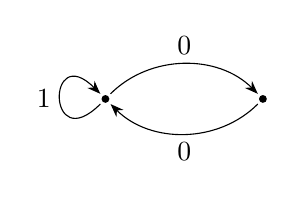
\begin{tikzpicture}
            [vertex/.style={circle, fill=black, inner sep=1pt},
             shorten <=1pt, shorten >= 1pt, >={Stealth[]}]
             

            \node[vertex] (A) at (0,0) {};
            \node[vertex] (B) at (2,0) {};
    
            \path [->] (A) edge[out=225, in=135, distance=10mm] node[left] {$1$} (A);
            \path [->] (A) edge[out=45, in=135] node[above] {$0$} (B);
            \path [->] (B) edge[out=225, in=-45] node[below] {$0$} (A);
        \end{tikzpicture} 
        \caption{}\label{evenshift}
    \end{subfigure}
    \begin{subfigure}{0.31\textwidth}
        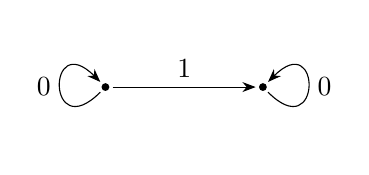
\begin{tikzpicture}
            [vertex/.style={circle, fill=black, inner sep=1pt},
             shorten <=1pt, shorten >= 1pt, >={Stealth[]}]
            \node[vertex] (A) at (0,0) {};
            \node[vertex] (B) at (2,0) {};
    
            \path [->] (A) edge[out=225, in=135, distance=10mm] node[left] {$0$} (A);
            \path [->] (A) edge node[above] {$1$} (B);
            \path [->] (B) edge[out=-45, in=45, distance=10mm] node[right] {$0$} (B);
        \end{tikzpicture} 
        \caption{}\label{010shift}
    \end{subfigure}

    \begin{subfigure}{0.31\textwidth}
        \begin{tikzpicture}
            [vertex/.style={circle, fill=black, inner sep=1pt},
             shorten <=1pt, shorten >= 1pt, >={Stealth[]}]
            \node[vertex] (A) at (0,0) {};
            \node[vertex] (B) at (2,0) {};
            \node[vertex] (C) at (2,2) {};
            \node[vertex] (D) at (0,2) {};
    
            \path [->] (A) edge[out=180, in=270, distance=10mm] node[left] {$1$} (A);
            \path [->] (C) edge[out=0, in=90, distance=10mm] node[right] {$1$} (C);
            \path [->] (A) edge node[below] {$0$} (B);
            \path [->] (B) edge node[right] {$0$} (C);
            \path [->] (C) edge node[above] {$0$} (D);
            \path [->] (D) edge node[left] {$0$} (A);

            % \draw[draw=none, use as bounding box] (0, 0) rectangle (3, -1);
        \end{tikzpicture} 
        \caption{}\label{nonminimaleven}
    \end{subfigure}
    \begin{subfigure}{0.31\textwidth}
        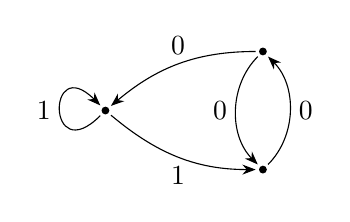
\begin{tikzpicture}
            [vertex/.style={circle, fill=black, inner sep=1pt},
             shorten <=1pt, shorten >= 1pt, >={Stealth[]}]
            \node[vertex] (A) at (0,0) {};
            \node[vertex] (C) at (2,.75) {};
            \node[vertex] (B) at (2,-.75) {};
    
            \path [->] (A) edge[out=225, in=135, distance=10mm] node[left] {$1$} (A);
            \path [->] (A) edge[out=-40, in=180] node[below] {$1$} (B);
            \path [->] (B) edge[out=45, in=-45] node[right] {$0$} (C);
            \path [->] (C) edge[out=225, in=135] node[left] {$0$} (B);
            \path [->] (C) edge[out=180, in=40] node[above] {$0$} (A);

            % \draw[draw=none, use as bounding box] (0, 0) rectangle (3, -1);
        \end{tikzpicture} 
        \caption{}\label{nondeterministiceven}
    \end{subfigure}
    \caption{Presentations of sofic shifts.}
\end{figure}

\begin{definition}
    Let \(\Gc = (G, \Lc)\) be a presentation of a sofic shift \(X\). For a vertex \(I \in \Vc_\Gc\), the 
    \term{follower set of \(I\)} is the set 
    \[F_\Gc(I) \triangleq \big\{ \; \Lc(\pi) : \pi \in \Bc(\shift{G}), i(\pi) = I \; \big\}.\]
    For a word \(w \in X\), the \term{follower set of \(w\)}
    is the set 
    \[F_X(w) \triangleq \big\{ \; u \in \Bc(X) : wu \in \Bc(X) \; \big\}.\]
\end{definition}

Let \(G\) and \(H\) be graphs. A \term{graph isomorphism between \(G\) and \(H\)}
is a pair of bijective functions \(\partial\Phi : \Vc_G \to \Vc_H\) and \(\Phi : \Ec_G \to \Ec_H\)
such that for all \(e \in \Ec_G\), we have \(\partial\Phi(i_G(e)) = i_H(\Phi(e))\)
and \(\partial\Phi(t_G(e)) = t_H(\Phi(e))\); i.e. \(G\) and \(H\) are the 
same graphs up to renaming the vertices and edges. Similarly, if \(\Gc\)
and \(\Hc\) are labeled graphs, then a \term{labeled-graph isomorphism from \(\Gc\) to \(\Hc\)}
is a graph isomorphism \((\partial\Phi, \Phi)\) between the underlying graphs of \(\Gc\)
and \(\Hc\) such that 
\(\Lc_\Hc(\Phi(e)) = \Lc_\Gc(e)\) for all \(e \in \Ec_\Gc\). We say 
\(\Gc\) and \(\Hc\) are \term{isomorphic} if there is an isomorphism between them.

A \term{minimal presentation} of a sofic shift \(X\) is a presentation 
of \(X\) with the smallest number of vertices among all presentations of \(X\). 
% Let \(\Gc\) be a presentation of a sofic shift. 
We say a presentation is \term{deterministic} if for each vertex in the presentation,
no two distinct edges starting at that vertex share the same label (i.e. the edges 
starting at that vertex are labeled uniquely). A presentation 
is \term{follower-separated} no pair of distinct vertices have the same follower 
sets (i.e. all the follower sets of the presentation are distinct). 

Every sofic shift has a deterministic presentation, which borrows the idea of the
\term{subset construction} from automata theory \cite{hopcroft2001introduction}.
In fact, \cite{jonoska1996sofic} showed that the minimal \term{deterministic finite 
automata} (DFA) accepting the 
language of a sofic shift has the minimal presentation for the 
sofic shift as a subgraph of the DFA. 

Additionally, every sofic shift has a follower-separated presentation. 
Any presentation can be made into a follower-separated by creating 
a graph from the equivalence class of follower sets (i.e. two vertices 
in a presentation are equivalent if they have the same follower set), 
and connecting any two equivalence classes if they have an edge 
between any of the vertices between the equivalence classes \cite{lind1995introduction}.
We call this process \term{follower-separation}.

\begin{example}
    As the vertex in the upper right of \Cref{nondeterministiceven} 
    is a vertex that has two edges starting at it labeled \(1\),
    this presentation is nondeterministic, but still presents 
    the even shift.
\end{example}

\begin{theorem}[name=\cite{lind1995introduction} Fundamental theorem of minimal deterministic presentations of irreducible sofic shifts]\label{fundamental}
    Let \(X\) be an irreducible sofic shift.
    \begin{enumerate}[(i)]
        \item Any minimal deterministic presentation of \(X\) is follower-separated and irreducible.
        \item Any two irreducible deterministic presentations of \(X\) 
        that are also follower-\\separated are isomorphic.
        \item Therefore, any two minimal deterministic presentations of \(X\) are isomorphic.
        \item Additionaly, a deterministic presentation, up to isomorphism, is the unqiue minimal deterministic presentation of \(X\)
        if and only if it is irreducible and follower-separated.
    \end{enumerate}
\end{theorem}

The idea of follower-separation once again borrows ideas from automata theory,
 as minimization of DFAs is done by creating a DFA from the equivalence class of states 
(defined in a similar manner). However, DFA minimization given the minimal 
DFA no matter what, but follower-separation does not necessarily yield a minimal 
presentation. It is only guaranteed to give the mininmal presentation if the 
original presentation is irreducible (\cite{lind1995introduction} Lemma 3.3.8).

\begin{example}
    The presentation in \Cref{nonminimaleven} is an irreducible presentation 
    of the even shift but is not follower-separated, so by \Cref{fundamental},
    it is not minmal. The presentation \Cref{evenshift} is an irreducible 
    follower-separated presentation of the even shift, so by \Cref{fundamental},
    it is minimal.
\end{example}

\begin{definition}
    Let \(\Gc\) be a presentation of a sofic shift \(X\), \(I\) be some vertex in \(\Gc\), and \(w \in \Bc(X)\).
    If every path \(\pi\) in \(\Gc\) that presents \(w\) ends at \(I\), then we say \term{\(w\) synchronizes to \(I\)}.
    We say that \(w\) is \term{synchronizing for \(\Gc\)} if it synchronizes to some vertex in \(\Gc\). 
    If there is a word that synchronizes to \(I\), then we say that the vertex \term{\(I\) is synchronizing}.
    Finally, we denote 
    \(S(\Gc)\) as the set of all synchronizing words for \(\Gc\).
\end{definition}

% We wrap up the preliminaries with relatively intuitive properties of follower 
% sets and synchronizing words.

% \begin{proposition}
%     Let \(\Gc\) be a a presentation of a sofic shift \(X\).
% \end{proposition}

\chapter{Irreducibility}

Consider the presentation in \Cref{reducibleevenshift}.
The shift presented by subgraph induced by \(I\) and \(J\) is the even shift, and every 
word presented by a path starting from \(K\) is presented by some path starting at 
\(I\) and \(J\). Hence, this presentation presents the even shift. Additionly, it is 
also follower-separated as \(01 \in F(K)\backslash F(I)\), \(1 \in F(K)\backslash F(J)\),
and \(1 \in F(I) \backslash F(J)\). 
When do follower-separated reducible presentations present irreducible shifts? We will first look 
at a simple class of reducible presentations.

\begin{figure}[h]
    \centering
    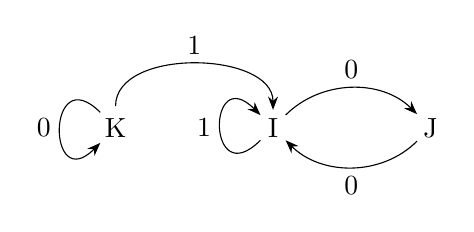
\begin{tikzpicture}
        [vertex/.style={circle, radius=10mm, inner sep=1pt},
         shorten <=1pt, shorten >= 1pt, >={Stealth[]}]
        \node[vertex] (A) at (0,0) {I};
        \node[vertex] (B) at (2,0) {J};
        \node[vertex] (C) at (-2, 0) {K};

        \path [->] (A) edge[out=225, in=135, distance=10mm] node[left] {$1$} (A);
        \path [->] (A) edge[out=45, in=135] node[above] {$0$} (B);
        \path [->] (B) edge[out=225, in=-45] node[below] {$0$} (A);
        \path [->] (C) edge[out=90, in=90] node[above] {$1$} (A);
        \path [->] (C) edge[out=135, in=225, distance=10mm] node[left] {$0$} (C);
    \end{tikzpicture} 

    \caption{A reducible, follower-separated presentation of the even shift}
    \label{reducibleevenshift}
\end{figure}

Given a graph and vertices \(I\) and \(J\) in the graph, we say \(I\) \term{communicates} with \(J\) if and only if 
\(I\) is reachable from \(J\) and \(J\) is reachable from \(I\). By saying 
a vertex is always reachable from itself, it is routine to check that this defines 
an equivalence relation. The equivalence classes are called \term{irreducible components},
as the subgraphs induced by each class are irreducible.

Let \term{\(\GtH\)} is an essential, deterministic, follower-separated presentation with two irreducible components
that induce two subgraphs, namely \(\Gc\) and \(\Hc\), such that there is 
exactly one edge starting in \(\Gc\) and ending in \(\Hc\). 
Some properties of \(\GtH\) are that the vertices of \(\Gc\) and \(\Hc\)
partition the vertices of \(\GtH\), both \(\Gc\) and \(\Hc\) are essential,  
any vertex in \(\Hc\) is reachable from any vertex in \(\GtH\), and no vertex in \(\Gc\) 
is reachable from any vertex in \(\Hc\). In this section, we will 
prove some properties of \(\GtH\).

\begin{figure}[h]
    \centering
    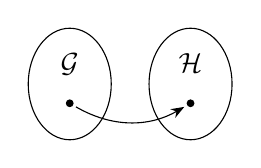
\begin{tikzpicture}[graph/.style={shape=ellipse, draw, minimum width=3em, text depth=1.5em},
                        dot/.style={shape=circle, fill, inner sep=1pt}]
        \node[graph] (G) at (0,0) {\(\Gc\)};
        \node[graph, right=of G] (H) at (0,0) {\(\Hc\)};
        \node[dot,below=-1.5em of G] (I) {};
        \node[dot,below=-1.5em of H] (J) {};
        \path [->] (I) edge[bend right, shorten <=1pt, shorten >= 1pt, >={Stealth[]}] node[above] {} (J);
    \end{tikzpicture}
    \caption{Representation of \(\GtH\).}
\end{figure}

% \begin{example}
%     The presentation in \Cref{reducibleevenshift} is \(\GtH\)-like, in the 
%     sense that it is essential, determinisitc, and has two irreducible components with only one edge 
%     between.  \(\Gc\) is the subgraph induced 
%     by \(K\) and \(\Hc\) is the subgraph induced by \(I\) and \(J\).
% \end{example}

\begin{proposition}\label{extensionthm}
    Every word \(u \in \Bc(\shift{\GtH})\) can be extended on the right to a 
    word \(u w \in \Bc(\shift{\GtH})\) that synchronizes to a vertex \(I\) in \(\Hc\).
\end{proposition}

\begin{proof}
    Let \(u \in \Bc(\shift{\GtH})\). As \(\GtH\) is deterministic and 
    follower-separated, then by \cite{lind1995introduction} Proposition 3.3.16, we can 
    extend \(u\) on the right to \(uw \in \Bc(\shift{\GtH})\) so that \(uw\)
    synchronizes to some vertex \(J\). As \(I\) is a vertex in \(\Hc\), 
    \(I\) can be reached from \(J\), so let \(v\) be  the label of a path 
    from \(I\) to \(J\). Then, \(uwv \in \Bc(\shift{\GtH})\) and any path presenting 
    \(uwv\) must end at \(J\), so \(uwv\) synchornizes to \(I\).
\end{proof}

\begin{corollary}\label{hsync}
    Every vertex in \(\Hc\) is synchronizing for \(\GtH\). 
\end{corollary}

\begin{proof}
    For a vertex \(I\) in \(\Hc\), take any word \(u \in \Bc(\shift{\GtH})\) and
    use \Cref{extensionthm} to synchronize it to \(I\). Hence, there is a word that synchronizes 
    to \(I\), so \(I\) is synchronizing.
\end{proof}

\begin{lemma}\label{wordlemma}
    Let \(u \in \Bc(\shift{\GtH})\). If \(u \notin \Bc(\shift{\Hc})\), then \(\shift{\GtH}\) is 
    reducible.
\end{lemma}

\begin{proof}
    By \Cref{extensionthm}, we can extend \(u\) on the right to a word \(uw \in \Bc(\shift{\GtH})\)
    so that any path presenting \(uw\) synchronizes to a vertex \(I\) in \(\Hc\). 
    We want to show that there is no word joining \(uw\) and \(u\). As \(uw\)
    synchronizes to \(I\), then by \cite{lind1995introduction} Lemma 3.3.15, \(F(I) = F(uw)\). 
    From the definition of irreducibility and follower sets of words, we 
    can see \(v\) is a word joining \(uw\) and \(w\)
    exactly when \(v \in F(uw)\) and \(u \in F(uwv)\).
    For any word \(v \in F(I)\), there is some path labeled \(v\) starting 
    at \(I\) and ending at \(J\) for some vertex \(J\) in \(\GtH\). Clearly,
    \(J\) is a vertex in \(\Hc\) as no vertex in \(\Gc\) is reachable from \(I\), so 
    \(F(J) \subseteq \Bc(\shift{\Hc})\).
    But \(u \notin \Bc(\shift{\Hc})\), so \(u \notin F(uwv)\). Thus, there is no word joining
    \(uw\) and \(u\), so \(\shift{\GtH}\) is reducible.
\end{proof}

\begin{theorem}\label{irreq}
    \(\shift{\GtH}\) is irreducible if and only if \(\shift{\GtH} = \shift{\Hc}\).
\end{theorem}

\begin{proof}
    Suppose \(\shift{\GtH}\) is irreducible, and let \(w \in \Bc(\shift{\GtH})\). By \Cref{wordlemma}, 
    as \(\shift{\GtH}\) is irreducible, then \(w \in \Bc(\shift{\Hc})\), so \(\Bc(\shift{\GtH}) \subseteq \Bc(\shift{\Hc})\).
    By construction of \(\GtH\), we have \(\Bc(\shift{\Hc}) \subseteq \Bc(\shift{\GtH})\). Therefore, 
    \(\Bc(\shift{\GtH}) = \Bc(\shift{\Hc})\) so \(\shift{\GtH} = \shift{\Hc}\).
    Conversely, suppose \(\shift{\GtH} = \shift{\Hc}\). As \(\shift{\Hc}\) is irreducible, then so 
    is \(\shift{\GtH}\).
\end{proof}

\begin{corollary}\label{irrsubshift}
    If \(\shift{\GtH}\) is irreducible, then \(\shift{\Gc} \subseteq \shift{\Hc}\).
\end{corollary}

\begin{proof}
    By \Cref{irreq}, if \(\shift{\GtH}\) is irreducible, then \(\shift{\GtH} = \shift{\Hc}\).
    As \(\shift{\Gc} \subseteq \shift{\GtH}\), then \(\shift{\Gc} \subseteq \shift{\Hc}\).
\end{proof}

\begin{theorem}\label{subshiftsyncequiv}
    \(\shift{\Gc} \subseteq \shift{\Hc}\) if and only if no vertex in \(\Gc\) is synchronizing for 
    \(\GtH\).
\end{theorem}

\begin{proof}
    Suppose \(\shift{\Gc} \nsubseteq \shift{\Hc}\). Then, there is a word \(w \in \Bc(\shift{\Gc})\) 
    but \(w \notin \Bc(\shift{\Hc})\). We can extend \(w\) to a word \(wu \in \Bc(\shift{\Gc})\) such 
    that \(wu\) is synchronizing for \(\Gc\). Therefore, every path in \(\GtH\) presenting \(wu\) 
    must be in \(\Gc\) as \(w \notin \Bc(\shift{\Hc})\), and as \(wu\) is synchronizing 
    for \(\Gc\), then it is synchronizing for \(\GtH\).

    Conversely, suppose there is a word \(w \in \Bc(\shift{\GtH})\) that synchronizes to a vertex in \(\Gc\).
    No path presenting this word can start in \(\Hc\) as no vertex in \(\Gc\) is reachable from any 
    vertex in \(\Hc\), so \(w \notin \Bc(\shift{\Hc})\). Clearly, \(w \in \Bc(\shift{\Gc})\) 
    as there is some path presenting \(w\) that starts and ends in \(\Gc\), so 
    \(\Bc(\shift{\Gc}) \nsubseteq \Bc(\shift{\Hc})\).
\end{proof}

\begin{corollary}\label{nogsync}
    If \(\shift{\GtH}\) is irreducible, then no vertex in \(\Gc\) is synchronizing for \(\GtH\).
\end{corollary}

\begin{theorem}
    \(\shift{\GtH} = \shift{\Hc}\) if and only if \(S(\GtH) \subseteq S(\Hc)\).
\end{theorem}

\begin{proof}
    Suppose \(\shift{\GtH} = \shift{\Hc}\). Let \(w \in B(\shift{\GtH})\) synchronize to some vertex \(I\)
    in \(\GtH\).
    If \(\pi\) is some path in \(\Hc\) presenting \(w\), then it must end at \(I\). By 
    \Cref{nogsync}, \(I\) cannot be a vertex in \(\Gc\), so it must be a vertex in \(\Hc\).
    Therefore, every path in \(\Hc\) presenting \(w\) ends at \(I\), so \(S(\GtH) \subseteq S(\Hc)\).

    Conversely, suppose \(S(\GtH) \subseteq S(\Hc)\). Let \(u \in \Bc(\shift{\GtH})\).
    By \Cref{extensionthm}, we can extend \(u\) to a word \(uw \in \Bc(\shift{\GtH})\) that 
    synchronizes to some vertex \(I\) in \(\GtH\). Hence, \(uw\) is synchronizing 
    for \(\GtH\), so it is also synchronizing for \(\Hc\). But if \(uw\) is synchronizing for
    \(\Hc\), then by definition, \(uw \in \Bc(\shift{\Hc})\). Therefore, \(\Bc(\shift{\GtH}) \subseteq \Bc(\shift{\Hc})\),
    so \(\shift{\GtH} = \shift{\Hc}\).
\end{proof}

\begin{proposition}
    If \(w \in S(\GtH)\) but \(w \notin S(\Hc)\), then \(w \notin \Bc(\shift{\Hc})\). 
\end{proposition}

\begin{proof}
    As \(w \in S(\GtH)\), there is a vertex \(I\) in \(\GtH\) such that every path in 
    \(\GtH\) presenting \(w\) ends at \(I\).
    If \(w \notin S(\Hc)\), then either 
    \(w \notin \Bc(\shift{\Hc})\) or for every vertex \(J\) in \(\Hc\) there is a path
    in \(\Hc\) that presents \(w\) but does not end at \(J\). Hence if the latter 
    condition were true, then this implies there is a path in \(\Hc\) that presents \(w\) 
    and does not end at \(I\). But this path is also in \(\GtH\) and presents \(w\), so it 
    should end at \(I\), which is a contradiction. Therefore, \(w \notin \Bc(\shift{\Hc})\).
\end{proof}

% \begin{theorem}
%     \(\shift{\GtH}\) is irreducible if and only if \(\shift{\Gc} \subseteq \shift{\Hc}\) and for all vertices 
%     \(I\) in \(\Gc\) there is a word \(w\) and vertex \(J\) in \(\Hc\) such that \(\delta_\GtH(I, w) = \delta_\GtH(J, w)\).
% \end{theorem}

% \begin{proof}
%     Suppose \(\shift{\Gc} \subseteq \shift{\Hc}\) and for all vertices 
%     \(I\) in \(\Gc\) there is a word \(w\) and vertex \(J\) in \(\Hc\) such that \(\delta_\GtH(I, w) = \delta_\GtH(J, w)\).
%     Let \(w \in \Bc(\shift{\GtH})\) and \(\pi\) be a path in \(\GtH\) presenting \(w\). 
%     If \(\pi\) starts in \(\Hc\), then \(w \in \Bc(\shift{\Hc})\). Otherwise, \(\)
% \end{proof}

\chapter{Subshift testing}

In the previous section, we posited that if \(\shift{\GtH}\) is irreducible, then \(\shift{\Gc}\) is a subshift of \(\shift{\Hc}\) (\Cref{irrsubshift}),
Although this condition is not sufficient for irreducibility (for example, \Cref{010shift}, the presentation of the \(010\)-shift), algorithmically, we will show there is a 
polynomial-time algorithm for deciding this, which gives a direction in looking for 
a characterization of irreducibility conditional on this subshift property.

Let \(\Gc\) be a deterministic presentation and \(I\) be a vertex in \(\Gc\). 
As every edge starting at \(I\) is labeled uniquely, we can see 
that every path starting at \(I\) is also labeled uniquely. That is, to say, for paths 
\(\pi\) and \(\tau\) both starting at \(I\), if \(\Lc(\pi) = \Lc(\tau)\), then \(\pi = \tau\). We can 
define a partial \term{transition function} \(\delta_\Gc : \Vc_\Gc \times \Ac_\Gc^* \to \Vc_\Gc\) 
with \(\delta_\Gc(I, w) \triangleq J\) if there is a path \(\pi\) labeled \(w\) starting 
at \(I\) and ending at \(J\) and \(\delta_\Gc(I, \epsilon) = I\) for all \(I\). However, if there is no path labeled \(w\) starting at \(I\),
then \(\delta_\Gc(I, w)\) is not defined, so in this case, we will say \(\delta_\Gc(I, w) \triangleq 0\),
where \(0\) is a constant distinct from the vertices of \(\Gc\). Additionally, we 
will define \(\delta_\Gc(0, w) = 0\). Finally, define 
the \term{subset transition function} \(\Delta_\Gc : \mathcal{P}(\Vc) \times \Ac_\Gc^* \to \mathcal{P}(\Vc)\)
with \(\Delta_\Gc(S, w) \triangleq \{ J \in \Vc_\Gc : J \neq 0 \text{ and } \delta_\Gc(I, w) = J \text{ for some } I \in S\}\).

\begin{proposition}\label{deltaprops}
    Let \(\Gc\) be an essential, deterministic labeled graph, and \(I\) and \(J\) be verticies in \(\Gc\). The following properties of the 
    transition function are true:

    \begin{enumerate}[(i)]
        \item \(w \in F(I)\) if and only if \(\delta_\Gc(I, w) \neq 0\)
        \item \(w \in \Bc(\shift\Gc)\) if and only if \(\Delta_\Gc(\Vc_\Gc, w) \neq \varnothing\)
        \item \(\delta_\Gc(I, uv) = \delta_\Gc(\delta_\Gc(I, u), v)\) for all vertices I in \(\Gc\) and \(u, v \in \Ac_\Gc^*\)
        \item \(\Delta_\Gc(S, uv) = \Delta_\Gc(\Delta_\Gc(S, u), v)\) for all subsets of vertices S of \(\Gc\) and \(u, v \in \Ac_\Gc^*\)
    \end{enumerate}
\end{proposition}

\begin{proof}
    Note that \(w \in F(I)\) exactly when there is a path labeled \(w\) starting at \(I\), so (i) follows 
    evidently from the defintion of \(\delta_\Gc\). Similarly, \(w \in \Bc(\shift{\Gc})\) exactly 
    when \(w \in F(I)\) for some vertex \(I\) in \(\Gc\), so (ii) follows from the definition of \(\Delta_\Gc\).

    For (iii), let \(u, v \in \Ac_\Gc^*\). If \(\delta_\Gc(I, uv) \neq 0\), then there is a unique path \(\pi=e_1 \dots e_n\) 
    labeled \(uv\) starting at \(I\) and ending at \(J\). As \(uv = \Lc(e_1) \dots \Lc(e_n)\), then for 
    nonempty \(v\), we can see that
    there is some \(i\) such that \(u = \Lc(e_1) \dots \Lc(e_i)\) and 
    \(v = \Lc(e_{i+1}) \dots \Lc(e_n)\)
    (for \(v = \epsilon\), what we are trying to show follows trivially). Let \(\rho_1 = e_1 \dots e_i\) and \(\rho_2 = e_{i+1} \dots e_n\).
    As \(\rho_1\) is a path starting at \(i(e_1)\) and ending at \(t(e_i)\) labeled \(u\),
    \(\delta_\Gc(I, u) = t(e_i)\). Similarly, as \(\rho_2\) is a path starting 
    at \(t(e_i)\) and ending at \(J\), \(\delta_\Gc(t(e_i), v) = J\). Therefore, 
    \(\delta_\Gc(\delta_\Gc(I, u), v) = J\). As there is a path labeled \(uv\)
    starting at \(I\) and ending at \(J\), then \(\delta_\Gc(I, uv) = J\). 
    
    If \(\delta_\Gc(I, uv) = 0\), 
    then there is no path labeled \(uv\) starting at \(I\). If there is no path 
    labeled \(u\) starting at \(I\), then \(\delta_\Gc(\delta_\Gc(I, u), v) = \delta_\Gc(0, v) = 0\).
    Otherwise, if there is a path labeled \(u\) starting at \(I\), then there must 
    be no path labeled \(v\) starting at \(\delta_\Gc(I, u)\), as otherwise, 
    \(\delta_\Gc(\delta_\Gc(I, u), v) \neq 0\) and then 
    \(\delta_\Gc(\delta_\Gc(I, u), v) = \delta_\Gc(I, uv) \neq 0\). Therefore, \(\delta_\Gc(\delta_\Gc(I, u), v) = 0\),
    which completes the proof for (iii). An similar argument to (iii)'s proof can be done applied to (iv).
\end{proof}

\begin{definition}
    Let \(\Gc\) be an essential, labeled graph. The \term{\(\Gc\) kill state graph with alphabet \(\Ac\)}
    is the labeled graph \(\Gc^0\) taking the same vertices and edges as \(\Gc\) with 
    an additional vertex \(0\) and edges such that for each \(a \in \Ac\) and vertex \(I\) in \(\Gc\),
    if there is no edge starting at \(I\) labeled \(a\), then there is an edge in \(\Gc^0\) 
    between \(I\) and \(0\) labeled a. Additionally, for each \(a \in \Ac\), there is an 
    edge from \(0\) to \(0\).
\end{definition}

From the definition of \(\Gc^0\), we can see that for 
all vertices \(I\) in \(\Gc\), \(w \in F(I)\) if and only if 
there is no path labeled \(w\) starting at \(I\) and ending at \(0\).

\begin{definition}
    Let \(\Gc\) and \(\Hc\) be labeled graphs. The \term{label product} of \(\Gc\) and \(\Hc\)
    is the labeled graph \(\Gc * \Hc\) such that if there is an edge \(e_1\) in \(\Gc\)
    between \(I_1\) and \(J_1\) and an edge \(e_2\) in \(\Hc\) between \(I_2\) and \(J_2\)
    with \(\Lc_\Gc(e_1) = \Lc_\Hc(e_2)\), then there is an edge in \(\Gc * \Hc\) between 
    \((I_1, I_2)\) and \((J_1, J_2)\) labeled \(\Lc_\Gc(e_1) = \Lc_\Hc(e_2)\).
\end{definition}

From the definition of \(\Gc * \Hc\), we can see that there is a word \(w\) and 
paths \(\pi\) in \(\Gc\) and \(\tau\) in \(\Hc\) both labeled \(w\) with
\(\pi\) starting at \(I_1\) and ending at \(J_1\) and \(\tau\) starting at \(I_2\)
and ending at \(J_2\)
if and only if there is a path in \(\Gc*\Hc\) starting at \((I_1, J_1)\) and 
ending at \((I_2, J_2)\).

With these two graph constructions, we can see that essential graphs \(\Gc\) and 
\(\Hc\) and for a vertex 
\(I\) in \(\Gc\) and a vertex \(J\) in \(\Hc\), checking \(F(I) \subseteq F(J)\)
reduces to checking the existence of a path in \(\Gc * \Hc^0\) from \((I, J)\) to 
any vertex in the set \(\{(K, 0) : K \in \Vc_\Gc\}\). With this, we 
can introduce \Cref{algsubshift}, which given an irreducible deterministic presentation \(\Gc\)
and an essential deterministic presentation \(\Hc\), test whether \(\Gc\)
presents a subshift of the shift \(\Hc\) presents. From a high 
level, the algorithm takes a vertex in \(\Gc\) and a vertex in \(\Hc\) and 
tries to find a word in the follower set of the vertex in \(\Gc\) but 
not in the follower set of the vertex in \(\Hc\). If it finds this word, 
the algorithm transitions the vertex in \(\Gc\) forward using the word and
transitions a subset of vertices in \(\Hc\) foward using the word. If 
the size subset of vertices from \(\Hc\) ever reaches \(0\), then 
the algorithm has found a word in \(\Bc(\shift{\Gc})\) not in \(\Bc(\shift{\Hc})\). 
Otherwise, if it does not find this word, then every word in \(\Bc(\shift{\Gc})\) must be in \(\Bc(\shift{\Hc})\).

\begin{algorithm}[H]
    \caption{Subshift testing}\label{algsubshift}
    \begin{algorithmic}[1]
        \Require $\Gc$ is an irreducible and deterministic presentation, $\Hc$ is an essential and deterministic presentation
        \Procedure{is\_subshift}{$\Gc, \Hc$}
                \State $I \gets$ any element in $\Vc_\Gc$
                \State $X \gets \Vc_\Hc$
                \State $w \gets \epsilon$
                \Repeat
                    \State $J \gets$ any element in $X$
                    \State find a word $u$ such that $\delta_\Gc(I, u) \neq 0$ and $\delta_\Hc(J, u) = 0$ 
                    \If{$u$ exists}
                        \State $w \gets wu$
                        \State $I \gets \delta_\Gc(I, u)$
                        \State $X \gets \Delta_\Hc(X, u)$
                        \If{$X = \varnothing$} 
                            \State \Return false
                        \EndIf
                    \EndIf
                \Until{$u$ does not exist}
            \State \Return true
        \EndProcedure
    \end{algorithmic}
\end{algorithm}

\begin{lemma}\label{invariants}
    If \(I_0\) is the value of \(I\) before entering the loop on lines 5-16, the invariants 
    \begin{enumerate}[(i)]
        \item \(\delta_\Gc(I_0, w) = I\)
        \item \(I \neq 0\)
        \item \(\Delta_\Hc(\Vc_\Hc, w) = X\)
    \end{enumerate}
    hold before the beginning of each iteration the loop. 
    Additionally, the loop always terminates.
\end{lemma}

\begin{proof}
    Clearly, \(I = I_0\) and \(w = \epsilon\) before entering the loop, so \(\Delta_\Gc(I_0, w) = \delta_\Gc(I, \epsilon) = I\).
    As \(I_0 \in \Vc_\Gc\), we have that \(I \neq 0\). Finally, as \(X = \Vc_\Gc\) before 
    entering the loop, \(\Delta_\Hc(\Vc_\Hc, w) = \Delta_\Hc(X, \epsilon) = X\), so the invariants hold 
    before entering the loop.

    Suppose the invariants were true before the current iteration of the loop and \(I\), \(J\), \(w\), and \(X\)
    had the values \(I_n\), \(J_n\), \(w_n\) and \(X_n\), respectively. Furthermore, suppose the loop does not exit
    after the current iteration. Because of this, then the algorithm must enter the 
    if statement on line 8 (and not enter the if statement on line 12), so there is a word \(u\) such that \(\delta_\Gc(I_n, u) \neq 0\)
    and \(\delta_\Hc(J_n, u) = 0\). We can see that \(w = w_n u\), \(I = \delta_\Gc(I_n, u)\), and 
    \(X = \Delta_\Hc(X_n, u)\) at the end of the current iteration, so from this, we can see 
    \[\delta_\Gc(I_0, w) = \delta_\Gc(I_0, w_n u) = \delta_\Gc(\delta_\Gc(I_0, w_n), u) = \delta_\Gc(I_n, u) = I\]
    and similarly,
    \[\Delta_\Hc(\Vc_\Hc, w) = \Delta_\Hc(\Vc_\Hc, w_n u) = \Delta_\Hc(\Delta_\Hc(\Vc_\Hc, w_n), u) = \Delta_\Hc(X_n, u) = X.\]
    Therefore, all the invariants hold before the next iteration of the loop.
    Finally, note that as \(\delta_\Hc(J_n, u) = 0\) and \(J_n \in X\), \(|X|\) is strictly less 
    than \(|X_n|\). This guarantees the loop terminates as if the exit condition is never 
    true, then \(|X| = 0\) will be true for some iteration so \(X = \varnothing\) and the algorithm exits on line 13. 
\end{proof}

\begin{theorem}
    \Cref{algsubshift} returns true if and only if \(\shift{\Gc} \subseteq \shift{\Hc}\).
\end{theorem}

\begin{proof}
    Suppose the algorithm returned false. If so, then it exited at line 13, so we 
    know \(X = \varnothing\). By \Cref{invariants}, \(\delta_\Gc(I_0, w) = I \neq 0\) so 
    \(w \in \Bc(\shift{\Gc})\) and \(\Delta_\Hc(\Vc_\Hc, w) = \varnothing\) so \(w \notin \Bc(\shift{\Hc})\).
    Therefore, \(\shift{\Gc} \nsubseteq \shift{\Hc}\). 

    Conversely, suppose \(\shift{\Gc} \nsubseteq \shift{\Hc}\). Then, there 
    is a word \(w \in \Bc(\shift{\Gc})\)
    but \(w \notin \Bc(\shift{\Hc})\). As \(w \in \Bc(\shift{\Gc})\), then \(\delta_\Gc(I^*, w) \neq 0\)
    for some vertex \(I^*\) in \(\Gc\), and as \(w \notin \Bc(\shift{\Hc})\), then 
    \(\delta_\Hc(J^*, w) = 0\) for all vertices \(J^*\) in \(\Hc\). Therefore, for 
    any value of \(I\), as \(\Gc\) is irreducible, there is a path 
    \(\pi\) starting at \(I\) and ending at \(I^*\), so 
    \[\delta(I, \Lc(\pi)w) = \delta_\Gc(\delta_\Gc(I, \Lc(\pi)), w) = \delta_\Gc(I^*, w) \neq 0\]
    and for any value of \(J\), \(\delta_\Hc(J, \Lc(\pi)w) = \delta_\Hc(\delta_\Hc(J, \Lc(\pi)), w) = \varnothing\).
    Hence, the algorithm can always find a word \(u\) on line 7. If the algorithm picks \(u\) to be \(\Lc(\pi)w\), 
    then the algorithm terminates, as \(\Delta_\Hc(\Vc_\Hc, \Lc(\pi)w) = \varnothing\).
    If not, then as discussed in \Cref{invariants}, the the current value of \(|X|\)
    is strictly less than the previous value of \(|X|\). Therefore, as the algorithm 
    can always find a word \(u\) on line 7, then \(|X| = 0\) eventually and 
    thus will return false eventually. 
\end{proof}

\begin{theorem}
    \Cref{algsubshift} can be computed in \(O(|\Vc_\Gc|\cdot|\Vc_\Hc|^3 + |\Ec_\Gc|\cdot|\Ec_\Hc|\cdot|\Vc_\Hc|)\) time.
\end{theorem}

\begin{proof}
    As \(|X|\) goes down by at minimum once every iteration of the loop, 
    and \(|X| = O(|\Vc_\Hc|)\), the loop repeats \(O(|\Vc_\Hc|)\) times. To compute line 7, 
    one can construct the graph \(\Gc * \Hc^0\) and and determine 
    if there is a path from \((I, J)\) to any vertex in the set 
    \(\{(K, 0) : K \in \Vc_\Gc\}\) using, say, a depth-first search.
    As \(|\Vc_{\Gc * \Hc^0}| = O(|\Vc_\Gc|\cdot|\Vc_\Hc|)\) and 
    \(|\Ec_{\Gc * \Hc^0}| = O(|\Ec_\Gc|\cdot|\Ec_\Hc|)\), then with 
    depth-first search, this step can be computed in \(O(|\Vc_\Gc|\cdot|\Vc_\Hc| + |\Ec_\Gc|\cdot|\Ec_\Hc|)\)
    time. As \(|u| = O(|\Vc_\Gc|\cdot|\Vc_\Hc|)\), computing \(\delta_\Gc(I, u)\) 
    takes \(O(|\Vc_\Gc|\cdot|\Vc_\Hc|)\) time. Similarly, computing 
    \(\Delta_\Hc(X, u)\) is reduces to computing \(\delta_\Hc\) at most \(|X|\) times, so 
    this can be computed in \(O(|\Vc_\Gc|\cdot|\Vc_\Hc|)\cdot O(|\Vc_\Hc|) = O(|\Vc_\Gc| \cdot |\Vc_\Hc|^2)\) time.
    In total, this is 
    \begin{align*}
        & O(|\Vc_\Hc|)\cdot \big( O(|\Vc_\Gc|\cdot|\Vc_\Hc| + |\Ec_\Gc|\cdot|\Ec_\Hc|) + O(|\Vc_\Gc|\cdot|\Vc_\Hc|) + O(|\Vc_\Gc|\cdot|\Vc_\Hc|^2)\big)
        \\ &= O(|\Vc_\Hc|)\cdot O(|\Vc_\Gc|\cdot|\Vc_\Hc|^2 + |\Ec_\Gc|\cdot|\Ec_\Hc|) \\ 
        &= O(|\Vc_\Gc|\cdot|\Vc_\Hc|^3 + |\Ec_\Gc|\cdot|\Ec_\Hc|\cdot|\Vc_\Hc|).
    \end{align*}
\end{proof}

\chapter{Discussion and future work}

Although the algorithm does not fully solve the problem of deciding 
the irreducibility problem, it does shed some light on a general minimization 
procedure. For a \(\GtH\)-like graph, if \Cref{algsubshift} returns 
false on inputs \(\Gc\) and \(\Hc\), then we actually know the presentation 
is \term{synchronizing}, meaning that every vertex is synchronizing.
As such, since \(\GtH\) is follower-separated, then by Corollary 5.4 of
\cite{jonoska1996sofic}, it is minimal.

Looking forwards, determining when \(\shift{\GtH}\) is irreducible when 
\(\shift{\Gc} \subseteq \shift{\Hc}\) intuitively seems to be linked 
with how to check if all words coming from \(\Gc\) link up ``properly''
with \(\Hc\). For example, in \Cref{reducibleevenshift}, this it is 
simple to see that \(\Gc\) links up with \(\Hc\) properly.
On the contrary, the presentation in \Cref{notevenshift} is similar 
to \Cref{reducibleevenshift} in that \(\shift{\Gc} \subseteq \shift{\Hc}\),
but connects to the wrong place in \(\Hc\), and fails to 
present the even shift, as it introduces the word 
\(101\) into the language.

\begin{figure}[h]
    \centering
    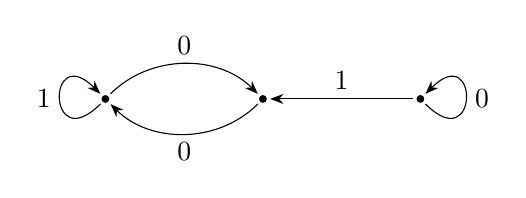
\begin{tikzpicture}
        [vertex/.style={circle, fill=black, inner sep=1pt},
         shorten <=1pt, shorten >= 1pt, >={Stealth[]}]
        \node[vertex] (A) at (0,0) {};
        \node[vertex] (B) at (2,0) {};
        \node[vertex] (C) at (4,0) {};

        \path [->] (A) edge[out=225, in=135, distance=10mm] node[left] {$1$} (A);
        \path [->] (A) edge[out=45, in=135] node[above] {$0$} (B);
        \path [->] (B) edge[out=225, in=-45] node[below] {$0$} (A);
        \path [->] (C) edge node[above] {$1$} (B);
        \path [->] (C) edge[out=-45, in=45, distance=10mm] node[right] {$0$} (C);
    \end{tikzpicture} 

    \caption{}
    \label{notevenshift}
\end{figure}

The results here are likely to be easily extended to presentations with arbitrarly 
many irreducible components. In fact, \cite{jonoska1996sofic} notes that 
for any presentation of an irreducible sofic shift, the subgraph 
induced by the synchronizing vertices presents the whole shift. In 
fact, this subgraph is irreducible and a sink (in the sense that 
there is no path starting at a vertex in the sink and ending 
in any other irreducible component). If given 
an arbitrary presentation that presents an irreducible shift, then 
to minimize it, one would need to find a synchronizing word and then 
identify the irreducible component it syncrhonizes to. Although not 
explicity discussed here, finding a syncrhonizing word should be doable in 
polynomial-time with a modification to \cite{eppstein1990reset}'s algorithm for 
finding a synchronizing word for DFAs.\footnote{
    Synchronizing words for DFAs, also known as reset words, differ slightly  
    from synchronizing words for presentations as the transition function 
    for DFAs is total to begin with, so the action of 
    taking the transition of the reset word takes you to the synchronizing 
    state no matter where you start, while for presentations, the action 
    of taking the transition of the synchronizing word either brings you 
    to \(0\) or the synchronizing state.
} Subshift testing can also be used for partial testing of the irreducibility 
of the shift a presentation presents. 
As each shift presented by an irreducible component is a subshift 
of the shift the whole presentation presents, it is easy to see that 
if a presentation presents an irreducible shift, then it is 
necessary that each irreducible component present a subshift of the 
synchronizing component. 

Finally, the hardness of the general problem of minimization seems 
to have not been investigated. Those familiar with 
automata theory can see that presentation of sofic shifts 
are closely related to \term{nondeterministic finite automata} (NFA),
as presentations can be interpreted as NFAs
by making the set of start states 
all the vertices of the presentation and 
every state a final state. If we restrict 
ourselves to deterministic presentations, then the only 
nondeterminism in the interpreted NFA is the multiple start states. 
In \cite{holzer2001state} and \cite{malcher2004minimizing}, 
minimization of a variant of a DFA 
that allows multiple start states (MDFA) is shown to be 
\(\mathsf{PSPACE}\)-complete in the former for the general case and
 \(\mathsf{NP}\)-complete in the latter for a restricted case.
Every presentation of a sofic shift gives a MDFA, but only ones
where every state is a final state. Further investigation should 
be done to see if this restriction affects the hardness of minimization.

\printbibliography


\end{document}